\chapter{\babTiga}
\label{bab:3}

\noindent\todo{
	jabarin sih isinya mau gmna
}

\section{Mekanisme \f{Attention}}
	\subsection{Attention sebagai \f{Dictionary Lookup}}

	Mekanisme \f{Attention} dapat ditinjau sebagai \f{Dictinoary Lookup}, yaitu untuk sebuah vektor kueri $\mathbf{q}$ dan sekumpulan pasangan terurut vektor $\mathcal{KV} = \{(\mathbf{k}_1, \mathbf{v}_2), (\mathbf{k}_2, \mathbf{v}_2), \dots, (\mathbf{k}_n, \mathbf{v}_n)\}$, mekanisme \f{attention} akan mengembalikan vektor nilai $\mathbf{v}_i$ yang memiliki vektor kunci $\mathbf{k}_i$ yang serupa dengan vektor kueri $\mathbf{q}$. \equ~\ref{equ:hard-attention-start} hingga \equ~\ref{equ:hard-attention-end} menunjukkan bagaimana mekanisme \f{attention} dilakukan.

\begin{align}
	\label{equ:hard-attention-start}
	\mathcal{KV} &= \{(\mathbf{k}_1, \mathbf{v}_2), (\mathbf{k}_2, \mathbf{v}_2), \dots, (\mathbf{k}_n, \mathbf{v}_n)\}, \\
	\text{tulis kembali }\mathbf{K}&= \begin{bmatrix}
		\mathbf{k}_1 \\
		\mathbf{k}_2 \\
		\vdots \\
		\mathbf{k}_n
	\end{bmatrix} \in \mathbb{R}^{n \times d_k}, \\
	\mathbf{V} &= \begin{bmatrix}
		\mathbf{v}_1 \\
		\mathbf{v}_2 \\
		\vdots \\
		\mathbf{v}_n
	\end{bmatrix} \in \mathbb{R}^{n \times d_v}, \\
	\text{Attention}(\mathbf{q}, \mathbf{K}, \mathbf{V}) &= \bm{\alpha}\mathbf{V} \in \mathbb{R}^{d_v},\\
	\bm{\alpha} &= [\alpha_{1}, \alpha_{2}, \dots, \alpha_{n}], \\
	\label{equ:hard-attention-end}
	\text{dengan } \alpha_i &= 
	\begin{cases}
	1, & \text{jika } i = \arg\max_{j} f_{attn}(\mathbf{q}, \mathbf{k}_j) \\
	0, & \text{lainnya}
	\end{cases}.
	\end{align}

	$f_{attn}(\mathbf{q}, \mathbf{k})$ adalah fungsi yang menghitung nilai keserupaan antara vektor kueri $\mathbf{q}$ dan vektor kunci $\mathbf{k}$. $\alpha_i$ pada persamaan di atas disebut sebagai bobot atensi dan nilai $f_{attn}(\mathbf{q}, \mathbf{k})$ disebut sebagai nilai atensi.

	Sebagai contoh, untuk $\mathbf{q}= [1,2]$, $\mathcal{KV} = \{([2,1],[1,0]), ([1,2],[0,1])\}$ serta fungsi $f_\text{attn}(\mathbf{q}, \mathbf{k}) =\mathbf{q}\cdot \mathbf{k}$, nilai dari $\text{Attention}( \mathbf{q}, \mathbf{K}, \mathbf{V})$ adalah $[0,1]$, karena nilai maksimal $f_\text{attn}$ terjadi ketika $\mathbf{k} = [1,2]$. 

	Mekansime \f{attention} pada \equ~\ref{equ:hard-attention-start} hingga \equ~\ref{equ:hard-attention-end} disebut sebagai \f{hard attention} karena hanya satu vektor nilai $\mathbf{v}_i$ yang dipilih dari sekumpulan vektor nilai $\mathbf{V}$. Berbeda dengan \f{hard attention} yang tidak terturunkan, \f{soft attention} mengambil seluruh vektor nilai $\mathbf{V}$ dan menghitung bobot $\alpha_i$ untuk setiap vektor nilai $\mathbf{v}_i$ dengan fungsi \f{softmax}. Hasil dari \f{soft attention} adalah rata-rata terbobot dari seluruh vektor nilai $\mathbf{V}$. \equ~\ref{equ:soft-attention-start} dan \pic~\ref{fig:soft-attention} menunjukkan bagaimana \f{soft attention} dilakukan.

	\begin{figure}
		\centering
		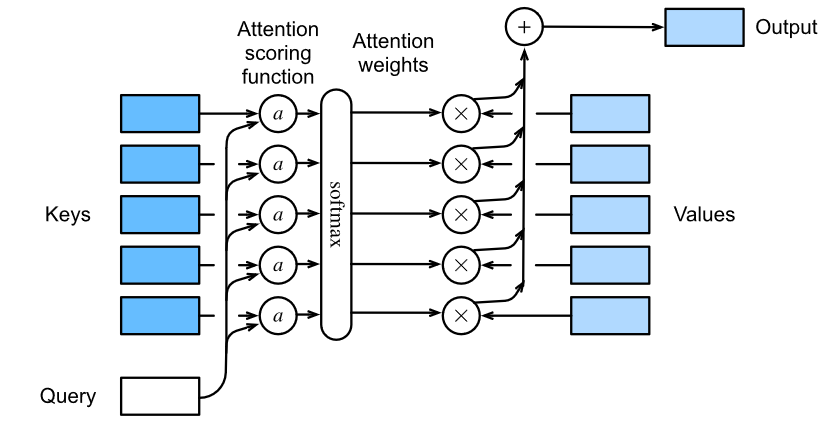
\includegraphics[width=1\textwidth]{assets/pics/softattention.png}
		\caption{Ilustrasi dari mekanisme \f{soft attention} \citep{zhang2023dive}}
		\label{fig:soft-attention}
	\end{figure}

	\begin{align}
		\label{equ:soft-attention-start}
		\text{Attention}(\mathbf{q}, \mathbf{K}, \mathbf{V}) &= \mathbf{\alpha}\mathbf{V} \in \mathbb{R}^{d_v},\\
		\text{dengan } \bm{\alpha} &= [\alpha_{1}, \alpha_{2}, \dots, \alpha_{n}], \\
		\text{dan } \alpha_{i}(\mathbf{q},\mathbf{k}_i) &= \text{Softmax}_i(\bm{\alpha}) = \frac{\exp(f_{attn}(\mathbf{q}, \mathbf{k}_i))}{\sum_{j=1}^{n} \exp(f_{attn}(\mathbf{q}, \mathbf{k}_j))}, \\
		\sum_{i=1}^{n} \alpha_{i} &= 1, \\
		\label{equ:soft-attention-end}
		0 \leq \alpha_{i} &\leq 1.
	\end{align}

	Dengan rata-rata terbobot dari $\mathbf{V}$, \f{soft attention} dapat dicari turunannya dengan \f{backpropagation} yang merupakan syarat \f{fundamental} yang harus dimiliki oleh sebuah model \f{deep learning}.

	Untuk contoh yang serupa dengan \f{hard attention},hasil dari $\text{Attention}(\mathbf{q}, \mathbf{K}, \mathbf{V})$ adalah $0.268 [1,0] + 0.732 [0,1] = [0.732, 0.268]$ dengan $\alpha_1 = \frac{\exp(4)}{\exp(4) + \exp(5)} \approx 0.268$ dan $\alpha_2 = \frac{\exp(5)}{\exp(4) + \exp(5)} \approx 0.732$.

	Pada kasus kumpulan kueri $\mathcal{Q} = \{\mathbf{q}_1, \mathbf{q}_2, \dots, \mathbf{q}_m\}$, Perhitungan atensi untuk setiap triplet $(\mathbf{q}_i, \mathbf{K}, \mathbf{V})$ dapat dihitung secara bersamaan dengan menggunakan operasi matriks. \equ~\ref{equ:soft-attention-start} hingga \equ~\ref{equ:soft-attention-end} yang digunakan untuk kasus 1 kueri dapat ditulis ulang seperti pada \equ~\ref{equ:soft-attention-matrix-start} hingga \equ~\ref{equ:soft-attention-matrix-end}.

	\begin{align}
		\label{equ:soft-attention-matrix-start}
		\text{tulis }\mathbf{Q} &= \begin{bmatrix}
			\mathbf{q}_1 \\
			\mathbf{q}_2 \\
			\vdots \\
			\mathbf{q}_m
		\end{bmatrix} \in \mathbb{R}^{m \times d_k}, \\
		\text{Attention}(\mathbf{Q}, \mathbf{K}, \mathbf{V}) &= \mathbf{A} \mathbf{V} \in \mathbb{R}^{m \times d_v},\\
		\mathbf{A} &= \begin{bmatrix}
			\bm{\alpha}_1 \\
			\bm{\alpha}_2 \\
			\vdots \\
			\bm{\alpha}_m
		\end{bmatrix} = \begin{bmatrix}
			\alpha_{11} & \alpha_{12} & \dots & \alpha_{1n} \\
			\alpha_{21} & \alpha_{22} & \dots & \alpha_{2n} \\
			\vdots & \vdots & \ddots & \vdots \\
			\alpha_{m1} & \alpha_{m2} & \dots & \alpha_{mn} \\
		\end{bmatrix} \in \mathbb{R}^{m \times n}, \\
		\label{equ:soft-attention-matrix-end}
		\alpha_{ij}(\mathbf{q}_i, \mathbf{k}_j) &= \text{Softmax}_j(\mathbf{\alpha}_i) = \frac{\exp(f_{attn}(\mathbf{q}_i, \mathbf{k}_j))}{\sum_{k=1}^{n} \exp(f_{attn}(\mathbf{q}_i, \mathbf{k}_k))},
	\end{align}

	dengan $\alpha_{ij}$ adalah bobot yang menunjukkan bobot atensi antara vektor kueri $\mathbf{q}_i$ dengan vektor kunci $\mathbf{k_j}$. 

	\subsection{Regresi Kernel Sebagai \f{Attention} non-parametrik}
	\label{sec:regresi-kernel}

	Salah satu pengunaan mekanisme \f{attention} terdapat pada regresi kernel, yang merupakan model statistik non-parametrik. \f{Attention} berubah menjadi regresi kernel dengan memilih fungsi keserupaan $f_{attn}(\mathbf{q}, \mathbf{k})$ menjadi fungsi non-parametrik $\mathcal{K}(\mathbf{q}, \mathbf{k})$, dan mengganti fungsi softmax menjadi fungsi normalisasi standar, seperti pada \equ~\ref{equ:regresi-kernel-end}.
	
	Pada model non-parametrik, model yang dibangun tidak memiliki parameter yang harus diestimasi atau dipelajari, melainkan model non-parametrik menggunakan seluruh atau sebagian dari \f{datasets} latih $\mathcal{D} = \{(\mathbf{x}_1, y_1), (\mathbf{x}_2, y_2), \dots, (\mathbf{x}_n, y_n)\}$ untuk memberikan prediksi $y_*$ untuk sebuah data uji $\mathbf{x}_*$. \equ~\ref{equ:regresi-kernel-start} hingga \equ~\ref{equ:regresi-kernel-end} menunjukkan bagaimana model regresi kernel melakukan prediksi $y_*$ untuk sebuah data uji $\mathbf{x}_*$.

	\begin{align}
		\label{equ:regresi-kernel-start}
		y_{*} = f(\mathbf{x}_{*}) &= \sum_{i=1}^{n} \alpha_{i}(\mathbf{x}_{*},\mathbf{x}_i) y_i, \\
		\label{equ:regresi-kernel-end}
		\text{dengan } \alpha_{i}(\mathbf{x}_{*},\mathbf{x}_i) &= \frac{\mathcal{K}(\mathbf{x}_{*},\mathbf{x}_i)}{\sum_{j=1}^{n} \mathcal{K}(\mathbf{x}_{*},\mathbf{x}_j)} \in [0, 1].
	\end{align}

	$\mathcal{K}(\mathbf{x}_{*},\mathbf{x}_i)$ adalah fungsi kernel (non-parametrik) yang menghitung keserupaan antara data uji $\mathbf{x}_{*}$ dengan data latih $\mathbf{x}_i$. \equ~\ref{equ:regresi-kernel-end} merupakan bentuk khusus dari mekansime \f{soft attention} \equ~\ref{equ:soft-attention-start}, dengan kueri $\mathbf{q}$ adalah data uji $\mathbf{x}_{*}$, kunci $\mathbf{k}_i$ adalah data latih $\mathbf{x}_i$, nilai $\mathbf{v}_i$ adalah $y_i$. \equ~\ref{equ:regresi-kernel-gaussian-start} menujukkan contoh kernel regresi dengan pemilihan kernel Gaussian $\mathcal{K}(\mathbf{x}_{*},\mathbf{x}_i) = \exp(-\frac{||\mathbf{x}_{*} - \mathbf{x}_i||^2 \beta}{2})$.

	\begin{align}
		\label{equ:regresi-kernel-gaussian-start}
		y_{*} = f(\mathbf{x}_{*}) &= \sum_{i=1}^{n} \alpha_{i}(\mathbf{x}_{*},\mathbf{x}_i) y_i	\\
		&= \sum_{i=1}^{n} \frac{\exp\left(-\frac{||\mathbf{x}_{*}-\mathbf{x}_i||^2 \beta^2}{2}\right)}{\sum_{j=1}^{n} \exp\left(-\frac{||\mathbf{x}_{*}-\mathbf{x}_j||^2 \beta^2}{2}\right)} y_i
	\end{align}

	\subsection{\f{Attention} Parametrik}

	Mekanisme \f{attention} yang dilakukan oleh \cite{transformerori} merupakan mekanisme \f{attention} parametrik. Salah satu alasan penggunaan $f_{attn}$ yang parametrik adalah pemilihan fungsi $f_{attn}$ yang non-parametrik seperti pada \sect~\ref{sec:regresi-kernel} memiliki kelemahan:


	\begin{enumerate}
		\item Relasi antar vektor kueri $\mathbf{q}$ dan vektor kunci $\mathbf{k}$ harus diketahui sebelumnya untuk memilih fungsi $f_{attn}$ yang tepat.
		\item Prediksi $y_*$ memerlukan seluruh data latih $\mathcal{D}$, $O(|\mathcal{D}|)$ komputasi diperlukan untuk melakukan satu prediksi.
	\end{enumerate}

	

	Pada mekanisme \f{attention} parametrik, nilai vektor kueri $\mathbf{q}$ dan $\mathbf{v}$ dibandingkan pada ruang vektor yang akan dipelajari (\f{learned embedding space}) daripada ruang vektor aslinya. Sebagai contoh, untuk suatu kueri $\mathbf{q}\in \mathbb{R}^{d_q}$, dan vektor kunci $\mathbf{k} \in \mathbb{R}^{d_k}$, \f{additive attention} yang diperkenalkan oleh \cite{bahdanau2016neural} menghitung nilai keserupaan antara $\mathbf{q}$ dan $\mathbf{k}$ seperti pada \equ~\ref{equ:additive-attention}

	\begin{align}
	\label{equ:additive-attention}
	f_{attn}(\mathbf{q} \mathbf{W}^q, \mathbf{k} \mathbf{W}^k) &= (\mathbf{q} \mathbf{W}^q  + \mathbf{k} \mathbf{W}^k)  \mathbf{W}^{\text{out}} \in \mathbb{R}, \\
	\text{dengan } &\mathbf{W}^q \in \mathbb{R}^{d_q \times d_{\text{attn}}}, \mathbf{W}^k \in \mathbb{R}^{d_k \times d_{\text{attn}}}, \mathbf{W}_{\text{out}} \in \mathbb{R}^{d_{\text{attn}} \times 1},
	\end{align}

	Dengan $\mathbf{W}^q$, $\mathbf{W}^k$, dan $\mathbf{W}^{\text{out}}$ adalah matriks parameter bobot yang akan diestimasi atau dipelajari selama proses pelatihan. Contoh parametrik \f{attention} yang lebih sederhana adalah \f{dot-product attention}. Fungsi $f_{attn}$ yang digunakan adalah perkalian titik antara $\mathbf{q}$ dan $\mathbf{k}$ di ruang vektor yang dipelajari (\f{learned embedding space}). \equ~\ref{equ:dot-product-attention} menunjukkan bagaimana \f{dot-product attention} dihitung.

	\begin{align}
		\label{equ:dot-product-attention}
		f_{attn}(\mathbf{q} \mathbf{W}^q, \mathbf{k} \mathbf{W}^k) = (\mathbf{q} \mathbf{W}^q) (\mathbf{k} \mathbf{W}^k)^{\top}\\
		\text{dengan } \mathbf{W}^q \in \mathbb{R}^{d_q \times d_{\text{attn}}}, \mathbf{W}^k \in \mathbb{R}^{d_k \times d_{\text{attn}}}.
	\end{align}

\section{Transformer}


	\begin{figure}
		\centering
		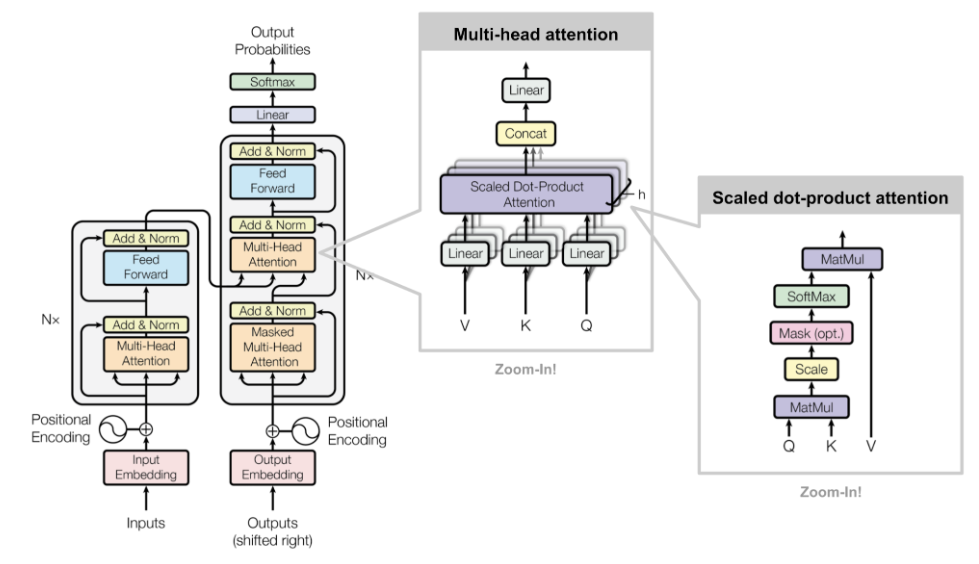
\includegraphics[width=1\textwidth]{assets/pics/lilianweng-transformer.png}
		\caption{Arsitektur \f{transformer} \citep{weng2018attention}.}
		\label{fig:transformer}
	\end{figure}

	\f{Transformers} merupakan Arsitektur \f{deep learning} yang pertama kali diperkenalkan oleh \cite{transformerori}. Awalnya Transformers merupakan model \f{sequance to sequance} yang diperuntukkan untuk permasalahan mesin translasi neural (\f{neural machine translation}). Namun, sekarang \f{transformer} juga digunakan untuk permasalahan pemrosesan bahasa alami lainnya. model-model yang berarsitektur \f{transformer} menjadi model \f{state-of-the-art} untuk permasalahan pemrosesan bahasa alami lainnya, seperti \f{question answering}, \f{sentiment analysis}, dan \f{named entity recognition}.
 
	Berbeda dengan arsitektur mesin translasi terdahulu, transformer tidak mengunakan \f{recurrent neural network} (RNN) atau \f{convolutional neural network} (CNN), melainkan transformer adalah model \f{feed foward network} yang dapat memproses seluruh \f{input} pada barisan secara paralel. Untuk menggantikan kemampuan RNN dalam mempelajari ketergantungan antar \f{input} yang berurutan dan kemampuan CNN dalam mempelajari fitur lokal, transformer bergantung pada mekanisme \f{attention}.

	Terdapat tiga jenis \f{attention} yang digunakan dalam model \f{transformer} \citep{transformerori}:
	\begin{enumerate}
		\item \f{Encoder self-attention}: menggunakan barisan \f{input} yang berupa barisan token atau kata sebagai masukan untuk menghasilkan barisan representasi kontekstual, berupa vektor, dari \f{input}. Setiap representasi token tersebut memiliki ketergantungan dengan token lainnya dari barisan \f{input}.
		\item \f{Decoder self-attention}: menggunakan barisan \f{target} yang berupa kalimat terjemahan parsial, barisan token, sebagai masukan untuk menghasilkan barisan representasi kontekstual (vektor) dari \f{target}. Setiap representasi token tersebut memiliki ketergantungan dengan token sebelumnya dalam urutan masukan.
		\item \f{Decoder-encoder attention}: menggunakan barisan representasi kontekstual dari \f{input}, dan barisan representasi kontekstual dari \f{target} untuk menghasilkan token berikutnya yang merupakan hasil prediksi dari model. Barisan \f{target} yang digabung dengan token hasil prediksi tersebut akan menjadi barisan \f{target} untuk prediksi selanjutnya.
	\end{enumerate}

	Arsitektur dari \f{transformer} mengimplementasikan struktur pasangan encoder-decoder. Aristektur dari \f{transformer} dapat dilihat pada \pic~\ref{fig:transformer}. Lapisan\f{encoder} berfungsi untuk memahami konteks suatu kata dalam dokumen atau kalimat, sementara lapisan \f{decoder} digunakan untuk menyelesaikan masalah translasi menuju bahasa berbeda. \sect~\ref{sec:token-embedding} hingga \sect~\ref{sec:encoder} menjelaskan arsitektur model \f{transformer} dan berbagai mekanisme yang menyusun model \f{transformer}, khususnya \f{transformer encoder} yang menjadi \f{building block} dari \f{Biderectional Encoder Representations from Transformers} (BERT).

	\subsection{\f{Token Embedding (Input Embedding)}}
	\label{sec:token-embedding}

	Perlu diingat kembali bahwa \f{input} dari \f{Attention} (dan tentunya \f{transformer}) adalah barisan vektor. Jika \f{Attention} ingin dapat digunakan pada permasalahan bahasa, barisan kata atau subkata (selanjutnya disebut token) harus terlebih dahulu diubah menjadi barisan vektor.

	Representasi vektor dari token yang paling sederhana adalah dengan \f{one-hot encoding}. Andaikan $\mathcal{T} = \{t_1, t_2, \dots, t_{|\mathcal{T}|}\}$ adalah semua kemungkinan token yang mungkin muncul dalam permasalahan bahasa yang ingin diselesaikan. Untuk sembarang barisan token $t = (t_{i_1}, t_{i_2}, \dots, t_{i_L})$, representasi vektor dari token $t_{i_j}$ adalah vektor $\mathbf{oh}_{i_j} = [0, \dots, 0, 1, 0, \dots, 0] \in \mathbb{R}^{|\mathcal{T}|}$, dengan nilai 1 pada indeks ke $j$ dan nilai 0 pada indeks lainnya. \f{One-hot encoding} tentunya memiliki kelemahan:

	\begin{enumerate}
		\item Vektor yang dihasilkan adalah \f{sparse vector}, dan ukuran vektor yang dihasilkan cukup besar, yaitu $|\mathcal{T}|$.
		\item Representasi token yang buruk. Operasi vektor yang dilakukan pada \f{one-hot encoding} tidaklah bermakna. Misalnya, Jarak antar token akan selalu sama pada \f{one-hot encoding}, yaitu $\sqrt{2}$.
	\end{enumerate}

	Untuk Mengatasi kekurangan dari representasi \f{one-hot encoding}, reprentasi yang digunakan adalah vektor padat yang akan dipelajari ketika proses pelatihan. Misalkan $\mathbf{E}_{\mathcal{T}} \in \mathbb{R}^{|\mathcal{T}| \times d_{\text{token}}}$ adalah matriks parameter yang merupakan representasi vektor padat dari seluruh token ada. \equ~\ref{equ:token-embedding-start} hingga \equ~\ref{equ:token-embedding-end} menunjukkan bagaimana representasi vektor dari barisan suatu token $t$ dihitung. 

	\begin{align}
		\label{equ:token-embedding-start}
		t &= (t_{i_1}, t_{i_2}, \dots, t_{i_L}), \\
		\mathbf{e}_{i_j} &= \mathbf{oh}_{i_j} \mathbf{E}_{\mathcal{T}} \in \mathbb{R}^{d_{\text{token}}}, \\
		\label{equ:token-embedding-end}
		\text{Embed}(t) &= \mathbf{E}_{t} = \begin{bmatrix}
			\mathbf{e}_{i_1} \\
			\mathbf{e}_{i_2} \\
			\vdots \\
			\mathbf{e}_{i_L}
		\end{bmatrix} \in \mathbb{R}^{L \times d_{\text{token}}}.
	\end{align}

	\subsection{\f{Scaled Dot-Product Attention}}
	\label{sec:scaled-dot-product-attention}
	\f{Scaled dot-product attention} adalah mekanisme \f{Attention} parametrik yang digunakan dalam \f{transformers}. \f{Scaled dot-product attention} menghitung keserupaan antara vektor kueri $\mathbf{q}$ dan vektor kunci $\mathbf{k}$ pada ruang vektor yang dipelajari (\f{learned embedding space}) dengan fungsi keserupaan $f_{attn}(\mathbf{q} \mathbf{W}^q, \mathbf{k}\mathbf{W}^k) $ adalah perkalian titik antara $\mathbf{qW}^q$ dan $\mathbf{kW}^k$ yang kemudian dibagi dengan $\sqrt{d_{attn}}$, seperti pada \equ~\ref{equ:scaled-dot-product-attention}.

	\begin{align}
		\label{equ:scaled-dot-product-attention}
		f_{attn}(\mathbf{q} \mathbf{W}^q, \mathbf{k} \mathbf{W}^k) &= \frac{\mathbf{q} \mathbf{W}^q (\mathbf{k} \mathbf{W}^k)^{\top}}{\sqrt{d_{attn}}} \in \mathbb{R}, \\
		\text{dengan } &\mathbf{W}^q \in \mathbb{R}^{d_q \times d_{\text{attn}}}, \mathbf{W}^k \in \mathbb{R}^{d_k \times d_{\text{attn}}}.
	\end{align}

	pembagian dengan $\sqrt{d_{attn}}$ dilakukan untuk menjaga variansi dari nilai atensi $\mathbf{q} \mathbf{W}^q (\mathbf{k} \mathbf{W}^k)^{\top}$ tetap serupa dengan variansi $\mathbf{qW}^q$ dan $\mathbf{kW}^k$. Tanpa pembagian $\sqrt{d_{attn}}$, variansi dari nilai atensi akan memiliki faktor tambahan $\sigma^2 d_{attn}$, seperti yang ditunjukkan pada \equ~\ref{equ:initialize-dot-product-attention} hingga \equ~\ref{equ:variance-dot-product-attention}.

	\begin{align}
		\label{equ:initialize-dot-product-attention}
		\mathbf{qW}^q \sim \mathcal{N}(0, \sigma^2) \text{ dan } \mathbf{kW}^k \sim \mathcal{N}(0, \sigma^2). \\
		\label{equ:variance-dot-product-attention}
		\text{Var}(\mathbf{qW}^q (\mathbf{kW}^k)^{\top}) = \sum_{i=1}^{d_{attn}} \text{Var}\left((\mathbf{qW}^q)_i ((\mathbf{kW}^k)^{\top}_i\right) = \sigma^4 d_{attn}.
	\end{align}
	
	Akibatnya, untuk nilai $d_{attn}$ yang cukup besar, akan terdapat satu elemen atensi acak $(\mathbf{qW}^q (\mathbf{kW}^k)^{\top})_i$ sehinnga $(\mathbf{qW}^q (\mathbf{kW}^k)^{\top})_i \gg (\mathbf{qW}^q (\mathbf{kW}^k)^{\top})_j$ untuk sembarang nilai atensi lainnya. Jika faktor $d_{attn}$ tidak dihilangkan, \f{softmax} dari nilai atensi akan jenuh ke 1 untuk satu elemen acak tersebut dan 0 untuk elemen lainnya. Akibatnya, gradien pada fungsi \f{softmax} akan mendekati nol sehingga model tidak dapat belajar parameter dengan baik. 

	Dengan \f{scaled dot product attention}, tidak ada faktor $d_{attn}$ pada variansi dari nilai atensi. faktor $\sigma^4$ pada \equ~\ref{equ:variance-scaled-dot-product-attention} tidak menjadi masalah karena inisialisasi bobot Kaiming dan \f{layer normalisasi} yang dijelaskan pada \sect~\ref{sec:kaiminginit} dan \sect~\ref{sec:layer-normalization} mengakibatkan $\sigma^2 \approx 1$ sehingga $\sigma^4 \approx \sigma^2 \approx 1$.

	\begin{align}
		\label{equ:variance-scaled-dot-product-attention}
		\text{(scaled dot product attention) }\text{Var}\left(\frac{\mathbf{qW}^q (\mathbf{kW}^k)^{\top}}{\sqrt{d_{attn}}}\right) = \frac{\sigma^4 d_{attn}}{d_{attn}} = \sigma^4
	\end{align}

	Terakhir, untuk kumpulan vektor kueri $\mathcal{Q} = \{\mathbf{q}_1, \mathbf{q}_2, \dots, \mathbf{q}_m\}$, dan kumpulan vektor kunci dan nilai $\mathcal{KV} = \{(\mathbf{k}_1, \mathbf{v}_2), (\mathbf{k}_2, \mathbf{v}_2), \dots, (\mathbf{k}_n, \mathbf{v}_n)\}$, \f{scaled dot product attention} dapat dihitung secara bersamaan seperti pada \equ~\ref{equ:scaled-dot-product-attention-matrix-start} hingga \equ~\ref{equ:scaled-dot-product-attention-matrix-end}.

	\begin{align}
	\label{equ:scaled-dot-product-attention-matrix-start}
	\text{Tulis Kembali } \mathbf{Q} &= \begin{bmatrix}
		\mathbf{q}_1 \\
		\mathbf{q}_2 \\
		\vdots \\
		\mathbf{q}_m \\
	\end{bmatrix} \in \mathbb{R}^{m \times d_{q}}, \\
	\mathbf{K} &= \begin{bmatrix}
		\mathbf{k}_1 \\
		\mathbf{k}_2 \\
		\vdots \\
		\mathbf{k}_n \\
	\end{bmatrix} \in \mathbb{R}^{n \times d_{k}}, \\
	\text{dan } \mathbf{V} &= \begin{bmatrix}
		\mathbf{v}_1 \\
		\mathbf{v}_2 \\
		\vdots \\
		\mathbf{v}_n \\
	\end{bmatrix} \in \mathbb{R}^{n \times d_{v}}, \\
	\label{equ:scaled-dot-product-attention-matrix-end}
	\text{Attention}(\mathbf{QW}^q, \mathbf{KW}^k, \mathbf{V}) &= \text{Softmax}( \frac{\mathbf{QW}^q (\mathbf{KW}^k)^{\top}}{\sqrt{d_{attn}}}) \mathbf{V} \in \mathbb{R}^{m \times d_{v}}, \\
	\text{dengan } \mathbf{W}^q &\in \mathbb{R}^{d_q \times d_{\text{attn}}}, \mathbf{W}^k \in \mathbb{R}^{d_k \times d_{\text{attn}}}.
	\end{align}

	\subsection{\f{Self-Attention}}


	\begin{figure}
		\centering
		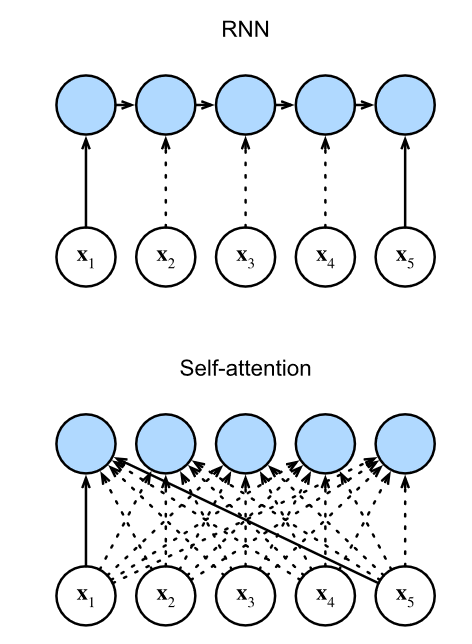
\includegraphics[width=1\textwidth]{assets/pics/rnn-compare-selfattention.png}
		\caption{Perbandingan RNN dan \f{self-attention} dalam menghasilkan representasi vektor kontekstual. Pada RNN, representasi vektor kontekstual setiap token bergantung pada perhitungan token sebelumnya. Pada \f{self-attention}, representasi vektor kontekstual setiap token dihitung secara independen dan paralel.}
		\label{fig:self-attention-rnn}
	\end{figure}

	\begin{figure}
		\centering
		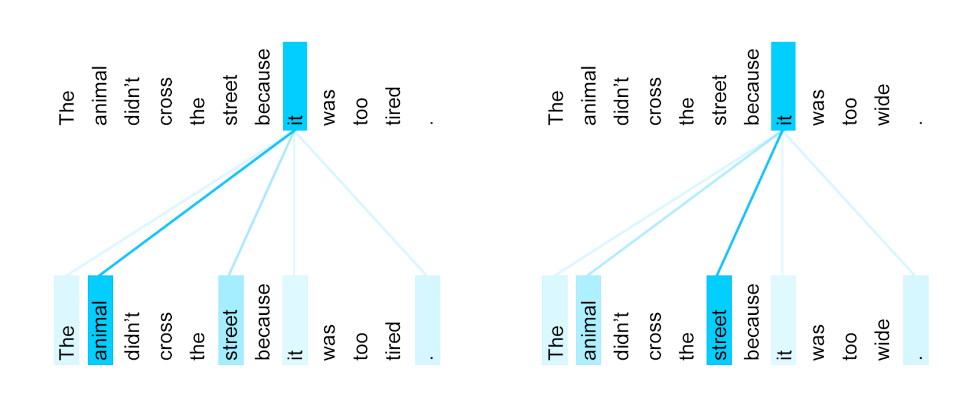
\includegraphics[width=1\textwidth]{assets/pics/self-attn-example.png}
		\caption{Ilustrasi \f{self-attention} dalam menghasilkan representasi vektor kontekstual dari barisan token. Representasi vektor dari token \f{it} akan bergantung terhadap barisan token \f{input}.}
		\label{fig:self-attention-example}
	\end{figure}

	\f{self-Attention layer} pada gambarxx adalah layer yang digunakan \f{transformer} untuk menghasilkan representasi vektor yang kontekstual dari barisan token input. Berbeda dengan RNN dalam menghasilkan representasi vektor kontekstual, \f{self-attention} tidak memerlukan ketergantungan sekuensial. Artinya representasi vektor kontekstual setiap tokennya dapat dihitung secara independen dan paralel.\pic~\ref{fig:self-attention-rnn} mengambarkan perbedaan kedua arsitektur dalam menghasilkan representasi vektor kontekstual. Kemampuan Paralelisme dari \f{self-attention} membuat proses komputasi menjadi lebih cepat pada \f{hardware} yang mendukung paralelisme. 

	Perhitungan \f{self-attention} pada \f{transformer} yang digunakan adalah \f{scaled dot product attention} yang telah dijelaskan pada \sect~\ref{sec:scaled-dot-product-attention}. Pada \f{self-attention}, vektor kueri $\mathbf{q}$, vektor kunci $\mathbf{k}$, dan vektor nilai $\mathbf{v}$ adalah vektor yang sama, yaitu \f{embedding} token $\mathbf{E}$ yang dijelaskan pada \sect~\ref{sec:token-embedding}. \equ~\ref{equ:self-attention-start} hingga \equ~\ref{equ:self-attention-end} menunjukkan bagaimana \f{self-attention} dihitung.

	\begin{align}
		\label{equ:self-attention-start}
		\text{Self-Attention}(\mathbf{E}) &= \text{Attention}(\mathbf{EW}^q, \mathbf{EW}^k, \mathbf{EW}^v) \\
		\label{equ:self-attention-end}
		&= \text{Softmax}(\frac{\mathbf{E} \mathbf{W}^q (\mathbf{E} \mathbf{W}^k)^{\top}}{\sqrt{d_{attn}}}) (\mathbf{E} \mathbf{W}^v) \in \mathbb{R}^{L \times d_{\text{attn}}}
	\end{align}

	\f{self-attention} dapat dikonsepsikan sebagai proses pembentukan represenatsi token yang kontekstual. untuk setiap tokennya, \f{self-attention} menghitung keserupaan antara token tersebut ($\mathbf{e}_{t_i} \mathbf{W}^q$) dengan seluruh token lainnya ($\mathbf{E} \mathbf{W}^k$) dengan \f{scaled dot product attention}. Hasil dari \f{scaled dot product attention} adalah vektor yang menunjukkan bobot atensi dari token tersebut terhadap token lainnya. Bobot atensi tersebut kemudian digunakan untuk menghitung rata-rata terbobot dari seluruh token lainnya ($\mathbf{E} \mathbf{W}^v$). Hasil dari rata-rata terbobot tersebut adalah representasi vektor kontekstual dari token tersebut. \pic~\ref{fig:self-attention-example} adalah contoh dari \f{self-attention} yang menghasilkan representasi vektor kontekstual pada token \f{it}. Pada \pic~\ref{fig:self-attention-example} kiri token \f{it} memiliki bobot atensi yang tinggi terhadap token dan \f{animal} sehingga representasi vektor kontekstual dari token \f{it} akan memiliki nilai yang serupa dengan representasi token \f{animal}. Di lain sisi, token \f{it} pada \pic~\ref{fig:self-attention-example} memiliki bobot atensi yang tinggi terhadap token \f{street}.
	
	\subsection{\f{Multi-Head Self-Attention}}
	
	\f{Multi-Head Attention} adalah arsiktetur \f{deep learning} yang melakukan mekanisme \f{attention} sebanyak
	
	
	\subsection{\f{Positional Encoding}}

	\subsection{\f{Position-wise Feed-Forward Network}}

	\subsection{Koneksi Residual dan \f{Layer Normalization}}
	\label{sec:layer-normalization}

	\subsection{Transformer Encoder}
	\label{sec:encoder}

\section{Bidirectional Encoder Representations from Transformers (BERT)}
	\subsection{Representasi Input}

	\subsection{Model Pralatih BERT}

		\subsubsection{\f{Masked Language Model}}

		\subsubsection{\f{Next Sentence Prediction}}

	\subsection{BERT untuk Bahasa Indonesia (IndoBERT)}

	\subsection{Penggunaan BERT untuk Pemeringkatan Teks}
		\subsubsection{$\text{BERT}_{\text{CAT}}$}

		\subsubsection{$\text{BERT}_{\text{DOT}}$}




